\documentclass[letterpaper,11pt,onecolumn]{article}
\author{D. Tork}
\title{My Learning in Quarantine}
\date{6 Aug 2020}

\usepackage{graphicx}
\graphicspath{ {./images/} }

\usepackage{url}

\begin{document}
\maketitle
\tableofcontents

\section{House Hunt}
Prior to the pandemic I had been writing a Python program to collect housing data in my area and
do some analysis to be a more informed buyer. I haven't purchased a home yet so my coding skills
are nothing to brag about, but it was truly a great learning experience. I was learning practical
coding, rather than printing \verb|hello world| or predicting flower species by the shapes of their
petals.

Amateur, pre-COVID me was scraping websites and storing my cleaned data in JSON files on my hard
drive. Quarantine me used the free account I had at \url{https://cloud.ibm.com} to start up a 
Cloudant database, a NoSQL document database based off of CouchDB. Cloudant isn't the top rated 
choice ever---it's new-ish, and its documentation is a little unclear at times and still being 
written---but its free offerings are generous (there are resource limits, such as 1GB of space and
20 reads/sec, 10 writes/sec, but I haven't come close to exceeding those) and the Lite account is 
perpetually free, not a trial period. 

The IBM docs were my \emph{only} resource for learning how to do the specific things like bulk
pushing, working within the Python API, and generally managing the database. This is because of a
severe lack of people asking or answering questions about Cloudant out in the Stack Exchange world,
or anywhere for that matter. It was to this difficulty I owe my progress I'm sure, because I had to
work overtime to try to understand their documentation and fit it to my use case. 


\section{Graph Databases}
Season 3 of Westworld began airing during quarantine, and I love to sink my teeth into a show that
I'm passionate about. So my lofty goal was to create a graph database of all the characters and 
entities in the show and their relationships, but without creating a single node or edge by hand. 
No, to make this worthwhile I was going to scrape the web for character data and parse episode
scripts to get connections between characters and maybe do some text analysis of all that
wonderfully deep dialogue.

The point at which my eyes became bigger than my stomach was when I described to a friend that, 
given that the season was all about not knowing who was actually in what body, I might be able to 
use data science to figure out whose pearl ended up in which host before the later episodes 
revealed it to us. The plan was to analyze hours of dialogue from seasons 1 and 2, establish a 
baseline for how each character speaks, then train a ML model to predict who was actually speaking.

I hardly got past the data cleansing stage. 

Not because I lost interest (still love the show, still love the idea), or because I hit
insurmountable technical roadblocks. It was simply that demands of my job pulled me away from
graph databases (which still have practical applications in our mission) and this project entered
the backlog. 

But before I stopped I managed to do two things. First, I gathered character data from the wiki
at https://westworld.fandom.com and cleaned it, which revealed a couple gaps and errors in some of
their data entry, which I promptly fixed much to the wiki admin's delight. Second, I did quite
a bit of research into different types of graph databases and data models. I grasped the concepts
well enough to sketch out a couple models to get me started.

\begin{center}
\end{center}

\begin{figure}[ht]
\centering

\textbf{**SPOILER WARNING**}

Don't look too closely at the following figure if you haven't watched \mbox{season 3.}

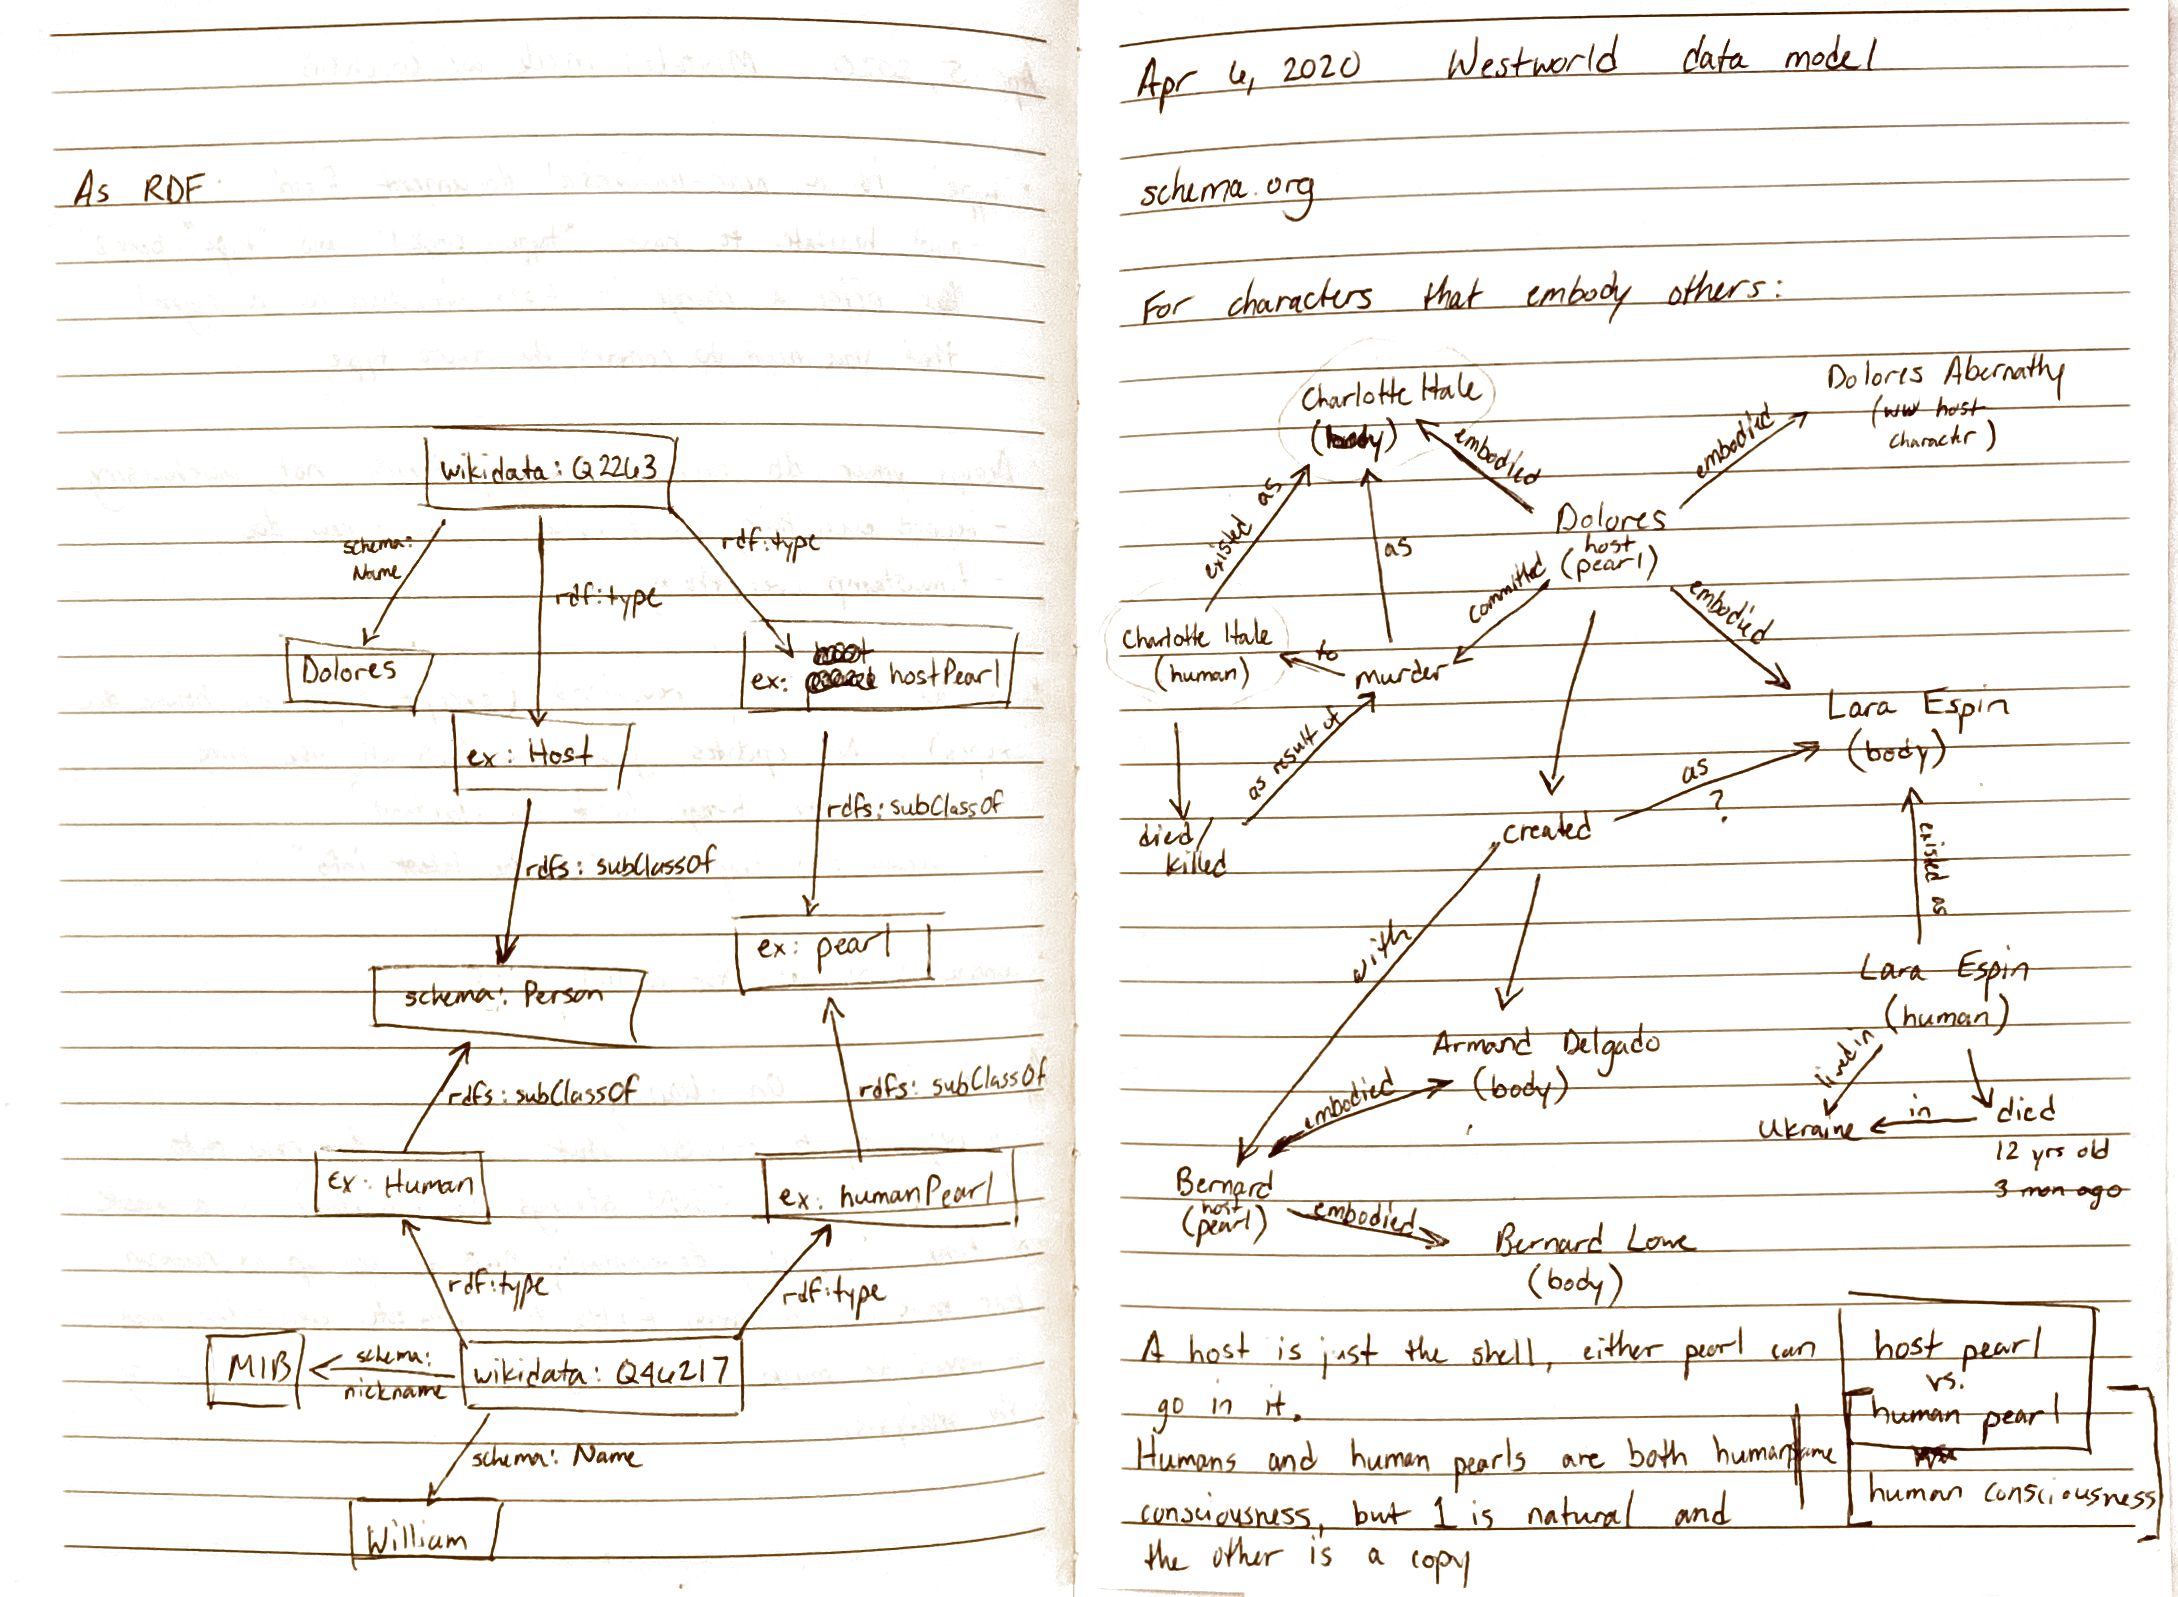
\includegraphics[width=\columnwidth]{westworld-notebook}
\caption{Westworld concepts as an Resource Description Framework (RDF, left) and a Labeled Property
Graph (right)}
\label{fig:notebook}
\end{figure}

This is something I will certainly return to, as it is a perfectly discrete project with which I 
can sharpen data analysis skills for the IC, should we need to continue spending time at home. You
can find my work (and contribute, if you'd like!) at \url{https://github.com/d-tork/violent-delights}.

\section{Raspberry Pi}
Already owned a raspberry pi, blah blah.

\section{ELK Stack}
We had Elasticsearch at work, so I got it at home.

But I wanted a cluster running all the time, yet not taking up my primary computer's resources.
So I turned an old Macbook Pro into an Ubuntu server.

\section{Ubuntu Server}

\section{Networking (Taking Control of My Router)}

Securing the servers and managing the ports and services taught me a lot about network 
infrastructure. And with this knowledge, I was finally confident enough to start opening up ports
in my router's firewall to show off some of my work to wonderfully supportive family members (they
had no idea what I was trying to show them, but were happy for me nonetheless, bless their hearts). 

\section{LaTeX}

Up ya game!

\end{document}
